\documentclass[conference]{IEEEtran}
\IEEEoverridecommandlockouts
% The preceding line is only needed to identify funding in the first footnote. If that is unneeded, please comment it out.
\usepackage{cite}
\usepackage{amsmath,amssymb,amsfonts}
\usepackage{algorithmic}
\usepackage{graphicx}
\usepackage{textcomp}
\usepackage{xcolor}
\usepackage{hyperref}
\def\BibTeX{{\rm B\kern-.05em{\sc i\kern-.025em b}\kern-.08em
    T\kern-.1667em\lower.7ex\hbox{E}\kern-.125emX}}
\begin{document}

\title{The Value of Forecasting: The Effect of Building Load Forecast Errors on the Performance of an Optimal Energy Management System \\
\thanks{This study was carried out in MESSI – Management Energy Systems for Smart Islands project, within the PRIN PROGETTI DI RICERCA DI RILEVANTE INTERESSE NAZIONALE – Bando 2022 and received funding from the European Union Next-GenerationEU (PIANO NAZIONALE DI RIPRESAE RESILIENZA - PNRR MISSIONE 4 COMPONENTE 2, INVESTIMENTO 1.1 –D.D. n. 104 del 02/02/2022, 2022HMYX2C). This manuscript reflects only the authors’ views and opinions, neither the European Union nor the European Commission can be considered responsible for them.}}

\author{\IEEEauthorblockN{Michael Wood}
\IEEEauthorblockA{Department of Energy\\
Politecnico di Milano\\
Milan, Italy\\
Email: michael.wood@polimi.it}
\and
\IEEEauthorblockN{Emanuele Ogliari}
\IEEEauthorblockA{Department of Energy\\
Politecnico di Milano\\
Milan, Italy\\
}
\and
\IEEEauthorblockN{Sonia Leva}
\IEEEauthorblockA{Department of Energy\\
Politecnico di Milano\\
Milan, Italy\\
}
}

\maketitle

\begin{abstract}
    Distributed renewable resources and microgrids will be a crucial technology during the energy transition. Fully utilizing these to reduce consumer electric costs will often necessitate forecasting electric load, required to solve the unit commitment problem. Traditional forecasting methods and also modern machine learning algorithms are often trained and evaluated on mean squared error, which may not be the best choice for designing forecasts that work effectively with a downstream decision maker: an optimal energy management system. This novel work constructs several different forecasts with different error distributions to study the error impact on simulated optimal battery dispatch in a building microgrid. The findings are that forecast error is most important during peak load periods and peak price periods, especially with consumer demand charges in place, and a zero-bias or random Gaussian error distribution is necessarily advantageous. 
    \end{abstract}

\begin{IEEEkeywords}
forecasting, optimization, error analysis, energy management, battery dispatch
\end{IEEEkeywords}

\section{Introduction}

Energy optimization relies heavily on accurate forecasts of electric load, dynamic prices, and renewable energy generation. From large power systems to small building microgrids, peak load events or sudden drops in solar generation can be mitigated with control actions such as demand response or dispatchable generation such as energy storage. However, depending on the control action, the cost of inaction, and other variables such as market opening and closing times, forecasting is required to anticipate the changes in load or generation, for instance by having enough State of Charge (SOC) in energy storage. %This forecast-response paradigm will be increasingly important as certain regions experience more extreme weather events, and renewable generation adds uncertainty to power systems and markets. 

In a forecast-and-optimizer Energy Management System (EMS) approach, errors in forecasts can significantly impact the performance of downstream decision-makers. Therefore this work simulates several statistically diverse forecasts in an optimal EMS to evaluate the effect of forecast error on the system's performance.

\subsection{Electric Load Forecasting}

Electric load forecasting is likely the oldest forecast in power systems. Recently short-term forecasts, on the order of hours to a few days, have been very important in supporting stable and efficient real-time market and operational decisions such as managing transmission congestion and informing market participants of their day-ahead bidding strategies. 

Techniques for load forecasting include traditional statistical methods such as SARIMA, but modern machine learning approaches like recurrent neural networks may improve typical error metrics as in \cite{wood2023day} and \cite{matrone2024electric}. Load forecasting errors can be inherent to the model or arise from various exogenous sources, including sudden weather changes, economic activities, and random anomalies in consumer behavior. In \cite{hong2016probabilistic} authors emphasize the importance of error decomposition, which involves breaking down the total forecast error into systematic and random components, to better understand and mitigate the sources of inaccuracies.

\subsection{Solar Power Forecasting}

Solar PV can be said to reduce the net load in many power systems because it is almost always dispatched immediately, having a near-zero marginal cost. Therefore a discussion of load forecasting errors should also consider solar PV forecast errors, which are affected by factors such as cloud cover, different types and elevations of clouds, temperature, wind, and electrical or mechanical phenomena in the PV system such as cell degradation and soiling \cite{leva2017analysis}. 

Statistical methods like ARIMA can be adapted for solar forecasting but often fall short in capturing the high variability. Instead, machine learning techniques, including ensemble methods and hybrid physically informed neural networks have shown improved performance as in \cite{yang2018history} and \cite{matera2024time}. 

\begin{figure}
    \centering
    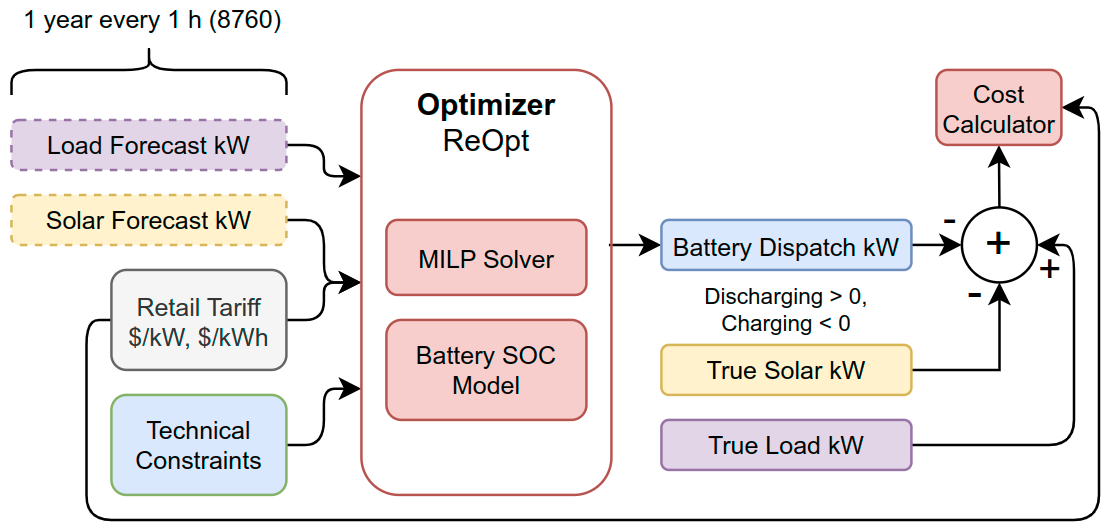
\includegraphics[width=1\linewidth]{images/flowchart.png}
    \caption{Simulation Flowchart}
    \label{fig:flowchart}
\end{figure}

\subsection{Error Analysis and Mitigation}

Error analysis involves assessing the forecast accuracy using metrics. Common deterministic forecasts are Mean Absolute Error (MAE), Mean Squared Error (MSE),  Mean Absolute Percentage Error (MAPE), and Mean Absolute Scaled Error (MASE), the last of which scales to a simple persistence benchmark. Rather for stochastic methods, metrics are required such as the Prediction Interval Coverage Probability (PICP) and Prediction Interval Normalized Average Width (PINAW).  A common problem is forecast bias, the tendency to have a non-zero mean for all forecasted values or just during certain intervals. Large errors are also caused by out-of-sample physical phenomena, such as grid outages or extreme weather events. Extreme magnitude clusters can have a large impact on the EMS performance and be difficult to predict, especially if the events are quite rare \cite{cirillo2020tail}.

Mitigating forecasting errors involves both improving forecast models and developing strategies to manage uncertainty. Analysis in \cite{makridakis2022predicting} of the M5 competition results show that the highest performance methods often use ensemble approaches, where multiple models are used to generate a range of possible outcomes, thus providing a measure of the forecast uncertainty. In \cite{grillo2012optimal} forecast uncertainty is mitigated with a strategy to minimize the starting SOC of a hot sodium nickel battery. Bayesian deep learning \cite{sun2019using} and approaches that consider decision-making under risk may aid the final EMS or decision-maker when the uncertainty is measurable.

\begin{figure}
    \centering
    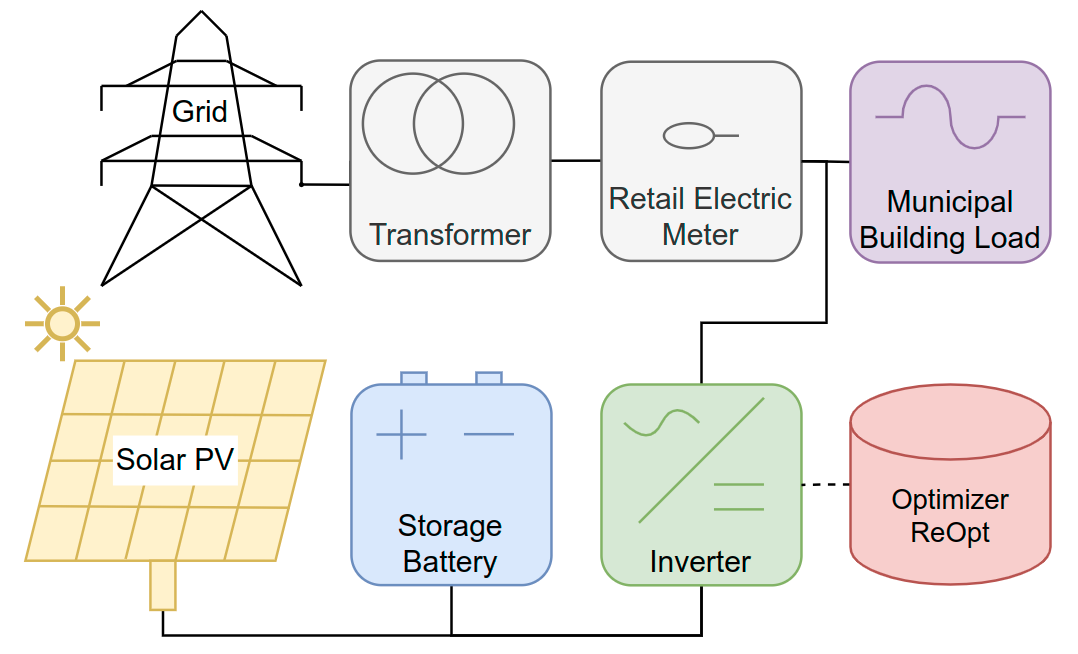
\includegraphics[width=.78\linewidth]{images/one-line.png}
    \caption{Site One-Line Diagram }
    \label{fig:one-line}
\end{figure}

This study's novel contribution to the literature is the approach of manually adding disturbances to the perfect forecast to create and study specific error distributions. The methodology is robust due to the use of true measured 1-minute interval electric load, true measured 1-minute solar PV production, a thoroughly validated optimal EMS (ReOpt by the National Renewable Energy Lab) \cite{simpkins2014reopt}, a true retail electric tariff, and two modified tariffs to study the effects of price structures on the results. Simulation code and data are published on GitHub for reproducibility.

The rest of the paper is organized as follows. In Methodology, the approach is described in detail. Next in Case Studies the specific problem and context are explained including data. Next Results are presented and discussed. And finally, Conclusions are drawn including the next steps for future work.

\begin{figure}
    \centering
    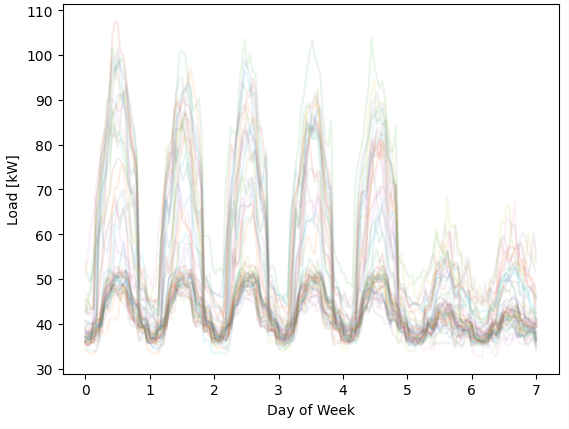
\includegraphics[width=1\linewidth]{images/weekly.png}
    \caption{Load Time Series}
    \label{fig:data-weekly}
\end{figure}
% The municipal building load overlaid weekly shows the daily seasonality, weekly seasonality, and much larger peaks which we confirm elsewhere to be during the summer months, and likely due to increased occupancy and air conditioning. The data is from one year of 1-minute interval average power measurements and is then mean downsampled to hourly for ReOpt.

\section{Methodology}

The study approach is a series of computer simulations that consist of two steps, graphically depicted in Fig.~\ref{fig:flowchart}. Each forecast-and-optimize simulation is performed on one year of time series data, solving the unit commitment problem for a behind-the-meter electric load, a co-located solar photovoltaic (PV) array, and a co-located storage battery. The only controllable asset is the storage battery, which can charge or discharge at any time step within its technical limits of maximum power and SOC. The following are some useful definitions:

\begin{itemize}
    \item Load consumption: $ L(i) \in \mathbb{R}_0^+ [kW]$
    \item Solar production: $ S(i) \in \mathbb{R}_0^+ [kW]$ 
    \item Battery charge, discharge: $ B_{c}(i), B_{d}(i) \in \mathbb{R}_0^+ [kW]$
    \item Battery net: $ B(i) \in \mathbb{R}  = B_{d} - B_{c}$
    \item Net load: $ L_{net} = L - S$
    \item Site load: $ L_{site} = L - S - B$
    \item True measured value: $ y_t(i) \in \mathbb{R}_0^+ $
    \item Forecasted value: $ y_f(i) \in \mathbb{R}_0^+ $
    \item Error: $ \epsilon \in \mathbb{R} = y_f - y_t $
    \item Time series interval: $ \Delta t \in \mathbb{R}^+ [h] $
\end{itemize} 


\subsection{Optimizer}

The unit commitment problem is solved by a centralized optimizer which is capable of modeling the the controllable assets, in this case only the battery. There are two different and important cases to consider:

\begin{enumerate}
    \item \textbf{Perfect Forecasting.} When the perfect load forecast (true measured load) and perfect solar forecast (true measured solar) are simulated, the result is the theoretical optimal battery dispatch for that year of load and solar measurements.
    \item \textbf{Imperfect Forecasting.} If instead an imperfect load and solar forecast are provided, the result is the optimal battery dispatch as if those forecasts were the true values. In other words, the simulation finds a global minimum of retail electric cost believing the forecasted load and solar to be true. Assuming that the battery dispatch is not modified by the EMS in the presence of information about the true measurements, the imperfect forecasts result in a retail electric cost that is necessarily greater than or equal to the theoretical optimal given perfect forecasting.
\end{enumerate}


\subsubsection{ReOpt}

The optimizer in this study is ReOpt, a techno-economic distributed energy resource (DER) planning tool, which is well-validated in the literature \cite{mishra2022computational}. It performs optimal operation and sizing of DERs, although it is not intended as a real-time optimal EMS. However, to optimally size DERs it must solve the unit commitment problem for one to several dispatchable DERs, which is the central task of an EMS. It does so by constructing and solving a mixed-integer linear program (MILP) which minimizes the life cycle cost of new and existing DERs from the perspective of the behind-the-meter DER owner. Binary decision variables are required, for instance, to prevent the battery from charging and discharging at the same time step.

Depending somewhat on the particular solver used, optimality of the solution is guaranteed for moderate complexity problem formulations due to a convex cost function and continuously differentiable, linear constraints \cite{ogunmodede2021optimizing}. Some disadvantages of ReOpt are the hourly interval which may contribute to errors relative to a real system (\cite{omoyele2024impact}), that forecasts cannot be updating in a rolling horizon manner, and some real-world losses are not considered such as battery heating and cooling.

ReOpt is both free and open source and is written using the JuMP library in the Julia programming language. It can be accessed accessed via an interactive web application, or a web API and Python script as in the case of this study.

\begin{figure}
    \centering
    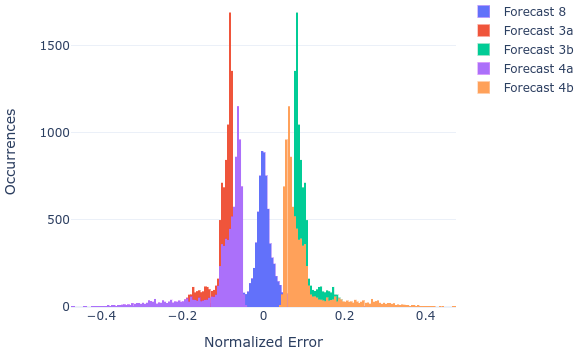
\includegraphics[width=1\linewidth]{images/hist.png}
    \caption{Error Distributions of Several Forecasts}
    \label{fig:hist}
\end{figure}

\subsection{Forecast Construction}

Rather than train various traditional and machine learning models to predict a time series, in this work the forecasts are manually manipulated starting from the true time series. In this way, the shape of the forecast error can be controlled and the effect on the EMS performance can be studied. 

\begin{enumerate}
\item One hypothesis is that errors during peak load periods are especially harmful to the EMS performance, especially when the rate tariff contains a price on peak demand, also called a demand charge.

\item A second hypothesis is that forecast errors during high energy prices are detrimental to EMS performance, especially in the absence of a demand charge.
\end{enumerate}

These hypotheses can be tested by manipulating the original load vector, which is a perfect forecast, with a disturbance that is proportional to the load magnitude, the load magnitude squared, energy prices, or demand prices. Table \ref{tab:forecasts} summarizes these constructed forecasts in rows 2 through 7, which are referenced as forecasts 2a through 7. Additionally, there is forecast 8 which is a seasonal persistence forecast where the lag value equals one week.

\begin{align}
    \text{nMAE } [\frac{kW}{kW}] = \frac{1}{N} \sum_{i=1}^N \frac{|y_f - y_t|}{max(y_t)} \label{eq:nmae} 
\end{align} 

A linear scaling factor $k$ is fit and applied separately to each forecast such that the normalized mean absolute error (nMAE) of each forecast is exactly 0.10. The value of 0.10 was determined experimentally to show a good spread of results: with an nMAE too low all the forecasts would be nearly perfect and indistinguishable, and vice versa.  The exceptions are that a perfect forecast will have an nMAE of zero, and a seasonal persistence forecast is possibly more interesting without other disturbances since it is already a good benchmark forecast \cite{hyndman2006another}. By forcing all the manipulated forecasts to have the same nMAE, any differences in the EMS performance can be attributed to the shape of the error distribution and not just the magnitude.

Because there are no regression or machine learning models to fit we don't separate the data into train, validation, and test subsets.

\begin{figure}
    \centering
    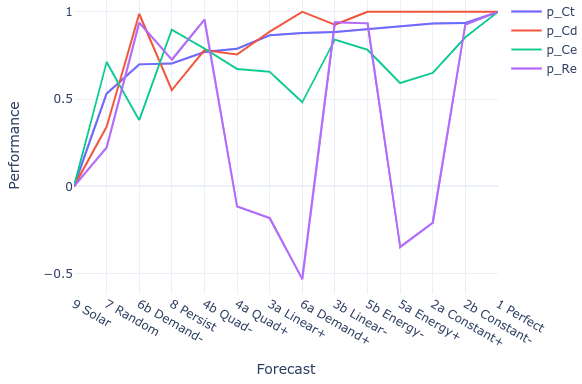
\includegraphics[width=1\linewidth]{images/perf_lines.png}
    \caption{Case Study 1 Performance}
    \label{fig:cs1-performance}
\end{figure}

\subsection{Performance Evaluation}

A premise of this work is that the utility of a distributed energy forecast should be determined by how much it reduces the final retail electric cost compared to a benchmark. The operational electric cost here is defined as what a customer would pay on a bill, less any fixed charges and particularly difficult-to-model components of the tariff, such as the rolling annual demand charge. Revenue from selling extra solar energy to the grid will be represented as a negative cost. Each timestep in $L_{site}$ belongs to exactly one time-of-use (TOU) period from 1 to $K$. Then each TOU period is assigned an energy buy price, demand charge price, and energy sell price. Equation \ref{eq:cost} calculates the dot product of in-TOU-period site loads and prices for each period, as well as the maximum monthly site load for each TOU period, which is multiplied by the TOU period's associated demand charge.

\begin{align}
    C_t,m           & = \sum_{k=1}^K [p_{d,k,m}  max(L^+_{site,k,m}) ...  \notag \\
                & +  \sum_{k=1}^K (p_{e,k,m} L^+_{site,k,m}\Delta t) ... \notag \\
                & +  \sum_{k=1}^K (p_{r,k,m} L^-_{site,k,m}\Delta t) ] \label{eq:cost} \\
                \text{where:}& \notag \\
                L_{site,k,m}^+(i) & \ge 0 \text{ and } L_{site,k,m}^-(i) \le 0\ \forall\ i \notag \\
                k & \text{: TOU period} \notag \\
                K & \text{: total TOU periods} \notag \\
                m & \text{: month} \notag \\
    C_t,m         & \in \mathbb{R}^+ [\$] \text{: total monthly retail electric cost} \notag \\
    p_{x,k,m}     & \in \mathbb{R}^+ [\$/kW] \text{ or } [\$/kWh] \text{: price for TOU } k \notag \\
    x \in & \{e:\text{energy},d:\text{demand},r:\text{revenue},t:\text{total} \}  \notag 
\end{align}


\begin{figure}
    \centering
    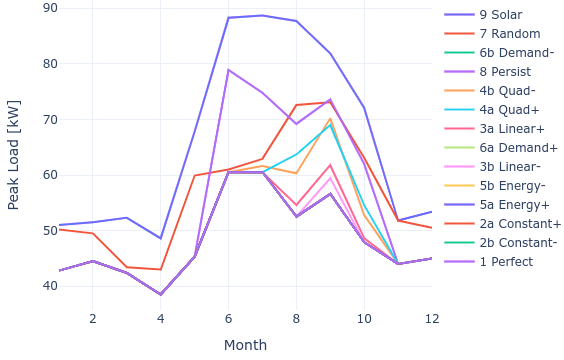
\includegraphics[width=1\linewidth]{images/monthly_peaks_lines.png}
    \caption{Case Study 1 Monthly Peaks}
    \label{fig:cs1-peaks}
\end{figure}

The two benchmarks in Table \ref{tab:forecasts} are forecast 1, the perfect forecast, and forecast 9, a solar-only benchmark, which has no battery. With no controllable DERs there are no decision variables and no forecasting to be done. The perfect forecast is a theoretical optimal (lowest cost) that can't be exceeded. The solar-only case should represent a low benchmark: an optimal EMS controlling a battery should be able to perform better than if the battery wasn't there at all.  

\begin{align}
    P(C_x) [\%]= & \frac{C_x - C_{x,perfect}}{C_{x,solar-only} - C_{x,perfect}} \times 100\% \label{eq:performance} \\
    \text{where:}& \notag \\
    C_x =& \text{ cost of forecast to be evaluated [\$]}  \notag \\
    C_{x,perfect} =& \text{ cost of perfect forecast [\$]}  \notag \\
    C_{x,solar-only} =& \text{ cost of solar-only benchmark [\$]}  \notag \\
    x \in & \{e:\text{energy},d:\text{demand},r:\text{revenue},t:\text{total} \}  \notag 
\end{align} 

These two book-end benchmarks suggest a normalized performance metric where a sample cost value $C$ lies in the range between the perfect forecast (1) and solar-only benchmark (9). This "performance" $P$ takes a value of 0\% when the forecast cost is equal to the solar-only benchmark and a value of 100\% when the forecast cost equals the theoretical optimal.

\begin{table}[t]
    \centering
    \caption{Forecasts and Solar-Only Benchmark}
    \label{tab:forecasts}
    \setlength{\tabcolsep}{9pt}
    \begin{tabular}{l l l l}
        %\hline
        Forecast               & Note                             & Definition & nMAE \\
        \hline
        \hline
        1 Perfect & Benchmark &  \(y_{perfect} = y_t\)        & 0.0               \\
        \hline
        2a Constant+ &             & \(y_f = y_t + k\)           & 0.1               \\
        2b Constant-  &            &  \(y_f = y_t - k\)           & 0.1               \\
        \hline
        3a Linear+     &           &  \(y_f = y_t + ky_t\)        & 0.1               \\
        3b Linear-      &          &  \(y_f = y_t - ky_t\)        & 0.1               \\
        \hline
        4a Quad+         &         &  \(y_f = y_t + ky_t^2\)      & 0.1               \\
        4b Quad-          &        &  \(y_f = y_t - ky_t^2\)      & 0.1               \\
        \hline
        5a Energy+ &Prices       &  \(y_f = y_t + kp_e\)        & 0.1               \\
        5b Energy- &Prices       &  \(y_f = y_t - kp_e\)        & 0.1               \\
        \hline
        6a Demand+ &Prices       &  \(y_f = y_t + kp_d\)        & 0.1               \\
        6b Demand- &Prices       &  \(y_f = y_t - kp_d\)        & 0.1               \\
        \hline
        7 Random &Gaussian      &  \(y_f = y_t + X\)            & 0.1               \\
        \hline
        8 Persist & 7 day               &  \(y_{persist} = y_t(i-168)\) & 0.033             \\
        \hline
        \hline
        9 Solar Only & Benchmark &  No forecast                  & n/a               \\
        \hline
    \end{tabular}
\end{table}

\begin{table}[t]
    \centering
    \caption{Retail Electric Tariff}
    \label{tab:tariff}
    \setlength{\tabcolsep}{3pt}
    \begin{tabular}{l l l l l}
        %\hline
        Period & Hours & Buy Prices & Buy Prices & Sell Price  \\
         &  & (Jun 1 - Sep 30) & (Oct 1 - May 31) & (all months) \\
        \hline
        \hline
        Off-peak & 0:00-9:00,  & 0.056 \$/kW  & 0.056 \$/kW & 0.050 \$/kWh \\
                  & 21:00-0:00 &              &        &       \\
        \hline
        Peak     & 9:00-21:00   & 0.075 \$/kWh, & 0.070 \$/kWh, & 0.050 \$/kWh \\
                 &              & 13 \$/kW & 11 \$/kW & \\
        \hline
    \end{tabular}
\end{table}

\begin{table}[t]
    \centering
    \caption{Case Studies}
    \label{tab:case-studies}
    \setlength{\tabcolsep}{6pt}
    \begin{tabular}{l l l}
        %\hline
        & Tariff & Modifications \\
        \hline
        \hline
        CS1 & Retail Electric Tariff (Table \ref{tab:tariff}) & \\
        CS2 & Retail Electric Tariff (Table \ref{tab:tariff}) & All \$/kW prices = 0  \\
        CS3 & Retail Electric Tariff (Table \ref{tab:tariff}) & Sell price = CA NEM3.0 \\
        \hline
    \end{tabular}
\end{table}

\begin{table}[t]%[!ht]
    \centering
    \caption{Case Studies 1-3: Forecasts vs Performance}
    \label{tab:performance}
    \setlength{\tabcolsep}{1.5pt}
    \begin{tabular}{l r r r r r r r r r r r}
        %\hline
        Forecast            & CS1      &          &          &               & CS2      &          &               & CS3      &          &          &               \\ 
        ~            & $P_{Ce}$ & $P_{Cd}$ & $P_{Re}$ & $P_{Ct}$      & $P_{Ce}$ & $P_{Re}$ & $P_{Ct}$      & $P_{Ce}$ & $P_{Cd}$ & $P_{Re}$ & $P_{Ct}$      \\ \hline \hline
        1 Perfect    & 100      & 100      & 100      & 100           & 100      & 100      & 100           & 100      & 100      & 100      & 100           \\ \hline
        2a Constant+ & 65     & 100     & -21    & \textbf{93} & 54     & -49    & 76          & 65     & 100     & -23    & \textbf{89} \\
        2b Constant- & 85     & 100     & 93     & \textbf{94} & 85     & 93     & 84          & 85     & 100     & 92     & \textbf{94} \\ \hline
        3a Linear+   & 66     & 89     & -18    & 87          & 55     & -45    & 77          & 66     & 89     & -19    & 82          \\
        3b Linear-   & 84     & 93     & 94     & 89          & 84     & 94     & 82          & 84     & 93     & 93     & \textbf{89} \\ \hline
        4a Quad+     & 67     & 76     & -12    & 79          & 58     & -36    & 78          & 67     & 76     & -12    & 75          \\
        4b Quad-     & 79     & 78     & 95     & 77          & 79     & 95     & 75          & 79     & 78     & 94     & 78          \\ \hline
        5a Energy+   & 59     & 100     & -35    & \textbf{92} & 44     & -75    & 69          & 59     & 100     & -37    & 87          \\
        5b Energy-   & 78     & 100     & 93     & 90          & 78     & 93     & 75          & 78     & 100     & 92     & \textbf{90} \\ \hline
        6a Demand+   & 48     & 00     & -53    & 88          & 100     & 100     & \textbf{100} & 48     & 100     & -57    & 82          \\
        6b Demand-   & 38     & 99     & 94     & 70          & 100     & 100     & \textbf{100} & 37     & 99     & 89     & 70          \\ \hline
        7 Random     & 71     & 34     & 22     & 53          & 67     & 10     & 79          & 73     & 21     & 25     & 45          \\ \hline
        8 Persist    & 90     & 55     & 73     & 70          & 87     & 65     & \textbf{92} & 90     & 55     & 73     & 70          \\ \hline
        9 Solar      & 0      & 0      & 0      & 0           & 0      & 0      & 0           & 0      & 0      & 0      & 0           \\ \hline
    \end{tabular}
\end{table}

\section{Case Studies}

Three case studies are built on the same building load data (Fig.~\ref{fig:data-weekly}) and are presented in Table \ref{tab:case-studies}, each with a different tariff structure but all with the same forecasts, benchmarks, and simulated DERs and site. The base tariff in Table \ref{tab:tariff} is only slightly simplified compared to the in vivo one, due to limitations of ReOpt in including a rolling annual demand charge on the cost function. This would only add marginally to the demand cost: 0.056 \$/kW compared to 11 and 13 \$/kW for Winter and Spring, respectively. In the second case study all demand charges are zeroed to see how errors affect the EMS in two very different objective functions: the first with a strong incentive to shave peaks, and the second not. In the third case study the demand charges are left intact but instead of a fixed solar sellback price of 0.05 \$/kWh, the California NEM3.0 price is used, which is a time-varying price based on the wholesale market price. Due to the famous duck curve and the need for late summer evening generation, prices in NEM3.0 can reach over 3 \$/kWh.

In all three case studies, only the load forecast is manipulated according to Table \ref{tab:forecasts}. Since solar PV has zero marginal cost it is always dispatched except for technical reasons for curtailment. Therefore the unit commitment problem can be reframed not as dispatching solar PV and storage to minimize the cost of electricity incurred by the load $L_{native}$, but instead as dispatching storage to minimize the cost of net load $L_{net}=L_{native}-S$. Now a positive error in the load forecast is identical to a negative error in the solar forecast, and vice versa. Furthermore, the combination of a positive load error and negative solar error can be reframed as the combined magnitude error in the net load.  

The nMAE of all forecasts is equal to 0.10 except for the perfect forecast which is 0, seasonal persistence which is 0.033, and the solar-only benchmark which has no forecast.

The site in the case studies is a medium-sized municipal building in northern Wisconsin, USA. The site has previously installed solar PV and energy meters which capture 1-minute time series data. For the purpose of this study, the battery and EMS are just abstractions. The simulations should somewhat accurately model power flows and battery charge and discharge of the site in Fig.~\ref{fig:one-line}. Conductor and transformer losses are estimated as a constant loss percentage, and real power reduction due to fluctuating power factors is not considered. 


\section{Results}

The error distributions in Fig.~\ref{fig:hist} reflect the intention to have different positive and negative forecast biases and to cluster the errors near peak values. In the 2a and 2b Constant forecasts, the errors take a single positive or negative value to the constant positive or negative offset (not shown in the image).

The final calculated costs for case study 1 in Fig.~\ref{fig:cs1-performance} (sorted in order of increasing $P_{Ct}$) show that demand cost $P_{Cd}$ is a good predictor of total cost. In fact, the Pearson correlation between the two is 0.94, whereas energy cost $P_{Ce}$ only correlates at 0.74 and revenue $P_{Re}$ is uncorrelated at 0.14. The Constant and Energy price forecasts are likely the best performing because both have fairly evenly distributed errors throughout the day, whereas Linear, Demand, and Quadratic forecasts focus the errors around load peaks or high demand prices.

An unexpected finding is that the worst-performing constructed forecast for a non-zero power price is the Random Gaussian disturbance ($P_{Cd}$ of 34\% in Table \ref{tab:case-studies}). This is due to the forecast not predicting many of the peak load events, any of which can set a fairly high peak of the month and therefore a high demand charge $C_d$ of the month. By comparison, the best-performing forecasts for $P_{Cd}$ (Cosntant +/-, Energy +/-, and Demand-) are those with the most constant error distributions in time, meaning that the forecasts temporally predict peaks well but not the magnitude. It's apparent from studying Fig.~\ref{fig:cs1-peaks} that the peak power is reduced (comparing Solar only to Perfect) by about 10 kW in winter and 20-30 kW in summer, which are not large values compared to the 100 kW 200 kWh battery simulated. The battery therefore has some buffer, or margin, available to effectively shave peaks as long as it is dispatched at 10-30 kW for a period that envelopes the true peak. This is to say that detecting the exact peak magnitude is not crucial to near-optimal demand charge reduction at this operating point. 

This is confirmed by case study 3 results, also deriving from a demand charge tariff, in Table \ref{tab:performance} where the Random forecast is again the worst performer. Both case studies 1 and 3 have the same four forecasts near or above 90\%: 2b Constant-, 2a Constant+, 5b Energy-, and 3b Linear-. Both case studies also have similar low performers: Random, Persist, and 6b Demand-, and in both forests the positive and negative bias forecasts don't show obvious trends.

In case study 2 there is no demand charge, and now the energy cost $P_{Ce}$ correlates with the total cost at 0.92. Without the demand charge, a forecast with errors concentrated around high demand prices should be relatively error-free during the other times of the day, and indeed the two best performing models are 6a and 6b Demand+ and Demand-. Persist performs above 90\% for the first time and Random is 79\%, suggesting both of those error shapes are harmful to peak shaving.


\section{Conclusions}

Analyzing and mitigating errors in electric load and solar forecasts are crucial for optimizing energy systems because of the decision maker downstream of the forecast. The initial investigation has discovered that several different load forecasts with identical nMAE can have extremely different performances in a simulated EMS. Advances in machine learning, synthetic data, and transfer learning offer promising improvements in forecast accuracy. However ongoing research is essential to develop the right forecasts and not generic ones, especially regarding peak shaving and peak load forecasting. An important finding is that a random Gaussian error distribution performs very poorly for a non-zero power price, suggesting that regression parameter fitting to minimize error in this way may suffer relative to other training or forecast methods.

The application of this work is in designing better forecasts for EMS operations. Whereas fitting SARIMA according to MSE could be effective in predicting day-ahead market prices, this study shows that a custom loss function should be used that emphasizes error reduction around peaks. Also, a given forecast with a higher statistical metric (such as MAE) might be preferable if the errors are more temporarily constant, even if there is non-zero bias. 

Some limitations of the study are: not including typical forecast models like regression or neural networks, not separately considering load and forecasting errors, using a single battery capacity, and not using a rolling horizon approach. Therefore future work will include various trained load and solar forecast models and a complete rolling-horizon optimal EMS. Future forecasting efforts will use tools like custom loss functions, Kalman filtering, and decision-making under risk approaches to tune the forecast in the direction that is optimal for the EMS to reduce costs, as well as investigate the role of load vs solar forecast errors. Finally, the cost of carbon should be considered in a multi-objective optimization in addition to economic cost.

\bibliographystyle{IEEEtran}
\bibliography{mendeley}

\end{document}
